%package list
\documentclass{article}
\usepackage[top=3cm, bottom=3cm, outer=3cm, inner=3cm]{geometry}
\usepackage{multicol}
\usepackage{graphicx}
\usepackage{url}
%\usepackage{cite}
\usepackage{hyperref}
\usepackage{array}
%\usepackage{multicol}
\newcolumntype{x}[1]{>{\centering\arraybackslash\hspace{0pt}}p{#1}}
\usepackage{natbib}
\usepackage{pdfpages}
\usepackage{multirow}    
\usepackage[normalem]{ulem}
\useunder{\uline}{\ul}{}
\usepackage{svg}
\usepackage{xcolor}
\usepackage{listings}
\lstdefinestyle{ascii-tree}{
    literate={├}{|}1 {─}{--}1 {└}{+}1 
  }

\lstset{basicstyle=\ttfamily,
  showstringspaces=false,
  commentstyle=\color{red},
  keywordstyle=\color{blue}
}
%\usepackage{booktabs}
\usepackage{caption}
\usepackage{subcaption}
\usepackage{float}
\usepackage{array}

\usepackage{enumitem}


\newcolumntype{M}[1]{>{\centering\arraybackslash}m{#1}}
\newcolumntype{N}{@{}m{0pt}@{}}


%%%%%%%%%%%%%%%%%%%%%%%%%%%%%%%%%%%%%%%%%%%%%%%%%%%%%%%%%%%%%%%%%%%%%%%%%%%%
%%%%%%%%%%%%%%%%%%%%%%%%%%%%%%%%%%%%%%%%%%%%%%%%%%%%%%%%%%%%%%%%%%%%%%%%%%%%
\newcommand{\itemEmail}{vmaldonadov@unsa.edu.pe}
\newcommand{\itemStudent}{Victor Gonzalo Maldonado Vilca}
\newcommand{\itemCourse}{Programación Web 2}
\newcommand{\itemCourseCode}{1702122}
\newcommand{\itemSemester}{III}
\newcommand{\itemUniversity}{Universidad Nacional de San Agustín de Arequipa}
\newcommand{\itemFaculty}{Facultad de Ingeniería de Producción y Servicios}
\newcommand{\itemDepartment}{Departamento Académico de Ingeniería de Sistemas e Informática}
\newcommand{\itemSchool}{Escuela Profesional de Ingeniería de Sistemas}
\newcommand{\itemAcademic}{2024 - A}
\newcommand{\itemInput}{Del 23 de mayo de 2024}
\newcommand{\itemOutput}{Al 8 de julio de 2024}
\newcommand{\itemPracticeNumber}{09}
\newcommand{\itemTheme}{Angular 1}
%%%%%%%%%%%%%%%%%%%%%%%%%%%%%%%%%%%%%%%%%%%%%%%%%%%%%%%%%%%%%%%%%%%%%%%%%%%%
%%%%%%%%%%%%%%%%%%%%%%%%%%%%%%%%%%%%%%%%%%%%%%%%%%%%%%%%%%%%%%%%%%%%%%%%%%%%

\usepackage[english,spanish]{babel}
\usepackage[utf8]{inputenc}
\AtBeginDocument{\selectlanguage{spanish}}
\renewcommand{\figurename}{Figura}
\renewcommand{\refname}{Referencias}
\renewcommand{\tablename}{Tabla} %esto no funciona cuando se usa babel
\AtBeginDocument{%
	\renewcommand\tablename{Tabla}
}

\usepackage{fancyhdr}
\pagestyle{fancy}
\fancyhf{}
\setlength{\headheight}{30pt}
\renewcommand{\headrulewidth}{1pt}
\renewcommand{\footrulewidth}{1pt}
\fancyhead[L]{\raisebox{-0.2\height}{
\includegraphics[width=3cm]{img/logo_episunsa.png}}}
\fancyhead[C]{\fontsize{7}{7}\selectfont	\itemUniversity \\ \itemFaculty \\ \itemDepartment \\ \itemSchool \\ \textbf{\itemCourse}}
\fancyhead[R]{\raisebox{-0.2\height}{
\includegraphics[width=1.2cm]{img/logo_abet}}}
\fancyfoot[L]{Victor M.}
\fancyfoot[C]{\itemCourse}
\fancyfoot[R]{Página \thepage}

% para el codigo fuente
\usepackage{listings}
\usepackage{color, colortbl}
\definecolor{dkgreen}{rgb}{0,0.6,0}
\definecolor{gray}{rgb}{0.5,0.5,0.5}
\definecolor{mauve}{rgb}{0.58,0,0.82}
\definecolor{codebackground}{rgb}{0.95, 0.95, 0.92}
\definecolor{tablebackground}{rgb}{0.8, 0, 0}

\lstset{frame=tb,
	language=bash,
	aboveskip=3mm,
	belowskip=3mm,
	showstringspaces=false,
	columns=flexible,
	basicstyle={\small\ttfamily},
	numbers=none,
	numberstyle=\tiny\color{gray},
	keywordstyle=\color{blue},
	commentstyle=\color{dkgreen},
	stringstyle=\color{mauve},
	breaklines=true,
	breakatwhitespace=true,
	tabsize=3,
	backgroundcolor= \color{codebackground},
}

\begin{document}
	
	\vspace*{10px}
	
	\begin{center}	
		\fontsize{17}{17} \textbf{ Informe de Angular 1 }
	\end{center}
	\centerline{\textbf{\Large Tema: \itemTheme}}
	%\vspace*{0.5cm}	

	\begin{flushright}
		\begin{tabular}{|M{2.5cm}|N|}
			\hline 
			\rowcolor{tablebackground}
			\color{white} \textbf{Nota}  \\
			\hline 
			     \\[30pt]
			\hline 			
		\end{tabular}
	\end{flushright}	

	\begin{table}[H]
		\begin{tabular}{|x{4.7cm}|x{4.8cm}|x{4.8cm}|}
			\hline 
			\rowcolor{tablebackground}
			\color{white} \textbf{Estudiante} & \color{white}\textbf{Escuela}  & \color{white}\textbf{Asignatura}   \\
			\hline 
			{\itemStudent \par \itemEmail} & \itemSchool & {\itemCourse \par Semestre: \itemSemester \par Código: \itemCourseCode}     \\
			\hline 			
		\end{tabular}
	\end{table}		
	
	\begin{table}[H]
		\begin{tabular}{|x{4.7cm}|x{4.8cm}|x{4.8cm}|}
			\hline 
			\rowcolor{tablebackground}
			\color{white}\textbf{Tarea} & \color{white}\textbf{Tema}  & \color{white}\textbf{Duración}   \\
			\hline 
			\itemPracticeNumber & \itemTheme & 2 horas   \\
			\hline 
		\end{tabular}
	\end{table}
	
	\begin{table}[H]
		\begin{tabular}{|x{4.7cm}|x{4.8cm}|x{4.8cm}|}
			\hline 
			\rowcolor{tablebackground}
			\color{white}\textbf{Semestre académico} & \color{white}\textbf{Fecha de inicio}  & \color{white}\textbf{Fecha de entrega}   \\
			\hline 
			\itemAcademic & \itemInput &  \itemOutput  \\
			\hline 
		\end{tabular}
	\end{table}
%%%%%%%%%%%%%%%%%%%%

  \section{Introducción}
  Angular es un framework desarrollado por Google para crear aplicaciones web y móviles robustas y escalables. 
  Se destaca por su arquitectura basada en componentes, enlace de datos bidireccional, y herramientas integradas 
  para manejar formularios, enrutamiento y optimización de rendimiento. Es ampliamente utilizado por su capacidad 
  de desarrollar aplicaciones de una sola página (SPAs) de manera eficiente y estructurada.

%%%%%%%%%%%%%%%%%%%%

  \section{Objetivos}
  \begin{itemize}
    \item Facilitar el desarrollo de aplicaciones de una sola página (SPA) con Angular.
    \item Mejorar la mantenibilidad y escalabilidad del código en Angular.
    \item Aumentar la productividad del desarrollador con Angular CLI y TypeScript.
    \item Implementar enlace de datos bidireccional eficiente en Angular.
    \item Ofrecer soporte robusto para formularios y validaciones en Angular.
    \item Optimizar el rendimiento de las aplicaciones web con Angular.
  \end{itemize}

%%%%%%%%%%%%%%%%%%%%
 
	\section{Tarea}
  \begin{itemize}
    \item Volver a implementar las clases teóricas en un proyecto en github realizando commits de cada avance.  
    \item Compartirlo con el profesor (usuario CarloCorrales010)
  \end{itemize}
  
%%%%%%%%%%%%%%%%%%%% 
 
  \section{Entregables}
  \begin{itemize}
    \item Informe hecho en Latex.
    \item URL: Repositorio GitHub.
  \end{itemize}
  
%%%%%%%%%%%%%%%%%%%%    
		
	\section{Equipos, materiales y temas utilizados}
  \begin{itemize}
    \item Angular
    \item Componentes
    \item Servicios
    \item Formularios
    \item Referencias
  \end{itemize}
 
%%%%%%%%%%%%%%%%%%%%

  \section{URL de Repositorio Github}
  \begin{itemize}
    \item Link Repositorio GitHub.
    \item \url{https://github.com/Victor-Gonzalo-Maldonado-Vilca/Angular.git}
  \end{itemize}

%%%%%%%%%%%%%%%%%%%%

  \section{Desarrollo del trabajo}
  
%%%%%%%%%%%%

  \subsection{Capturas de la Actividad}
  \begin{figure}[H]
    \centering
    \fbox{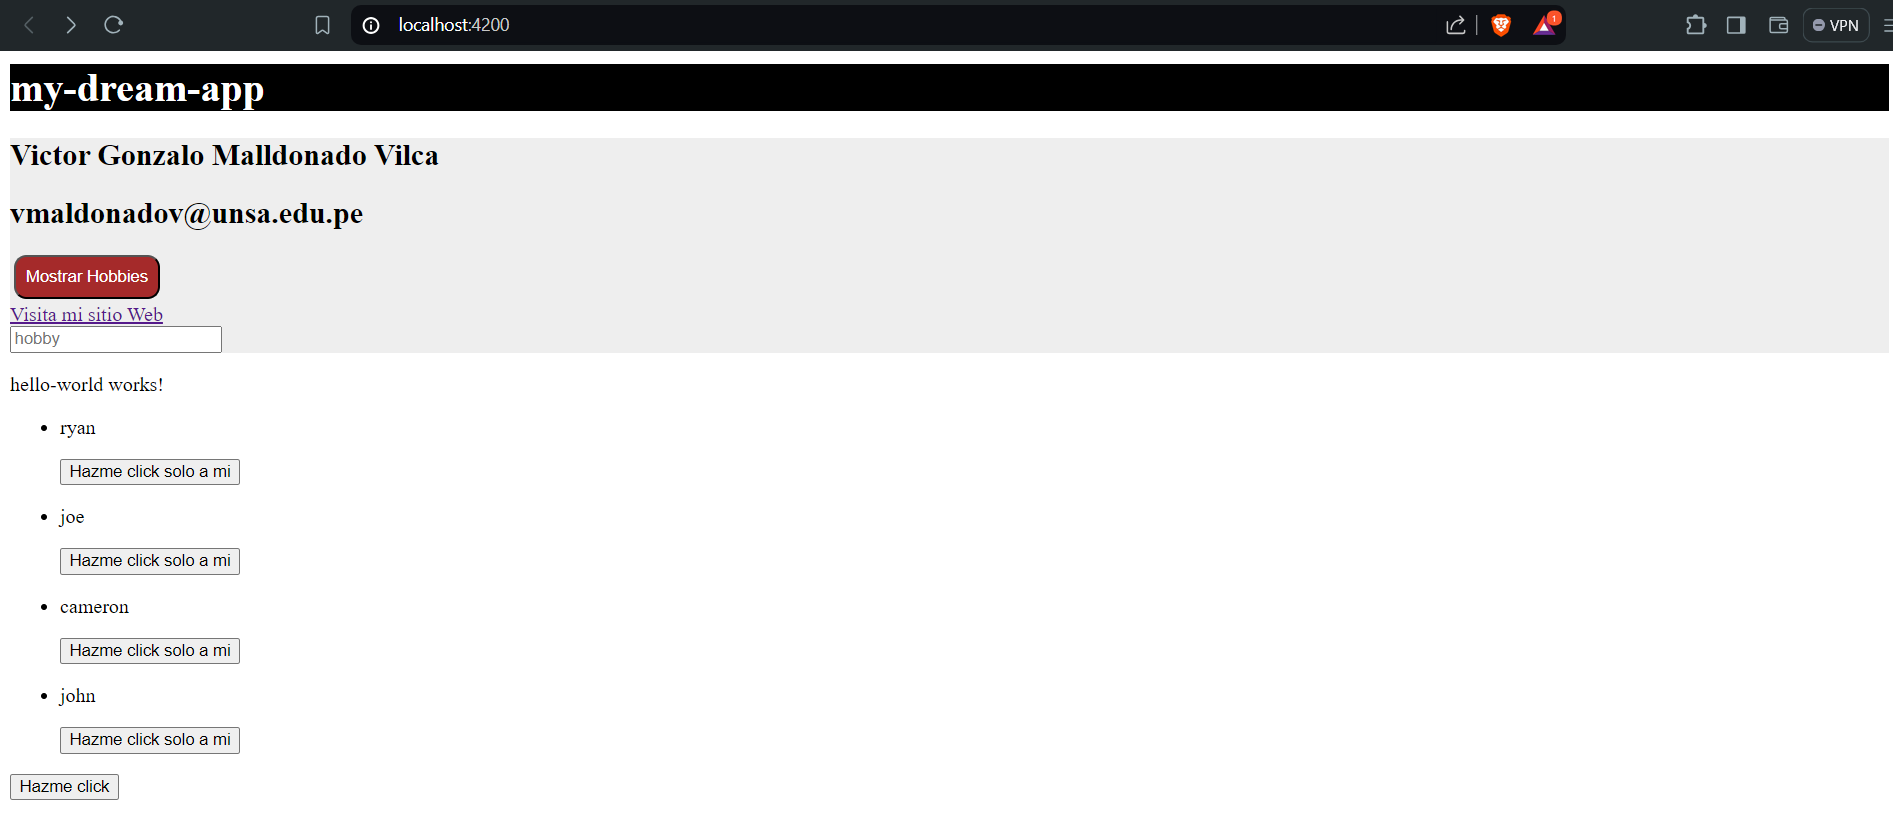
\includegraphics[width=1\textwidth, keepaspectratio]{img/ejecucion1.png}}
    \caption{Ejecución 1}
  \end{figure}
  \begin{figure}[H]
    \centering
    \fbox{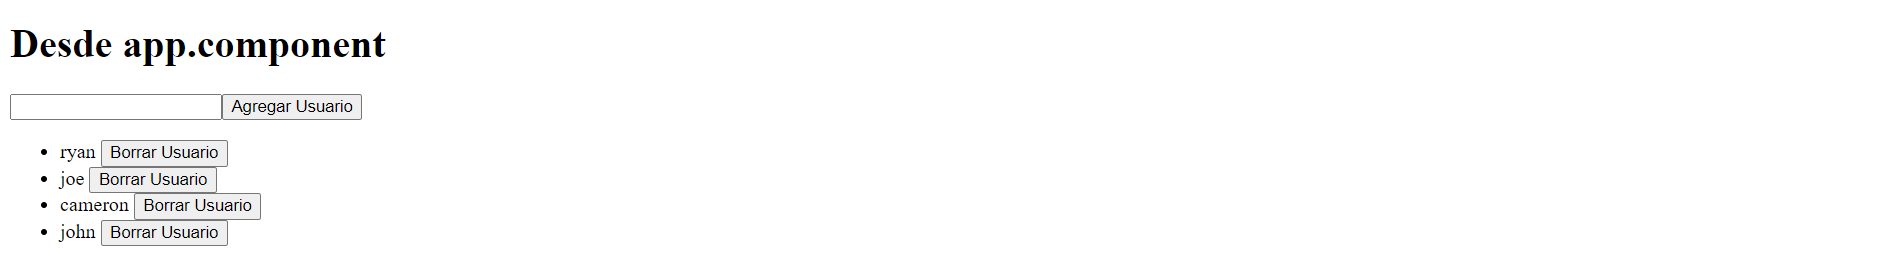
\includegraphics[width=1\textwidth, keepaspectratio]{img/ejecucion2}}
    \caption{Ejecución 2}
  \end{figure}
  \begin{figure}[H]
    \centering
    \fbox{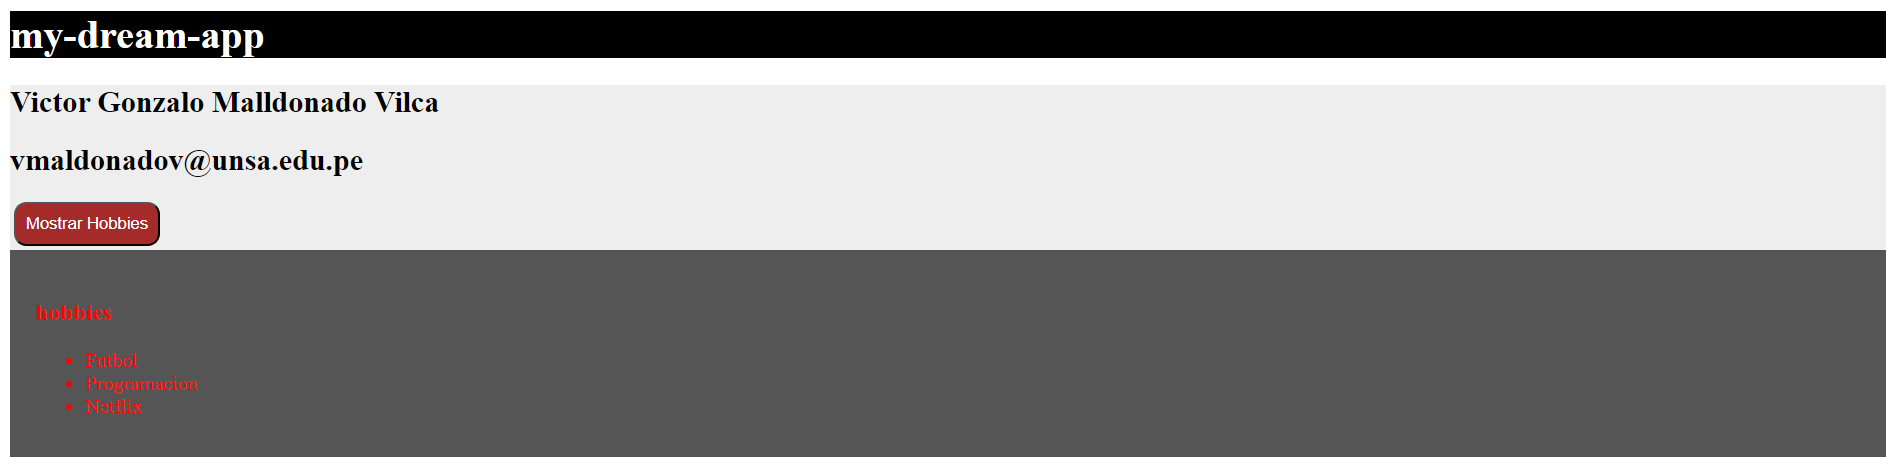
\includegraphics[width=1\textwidth, keepaspectratio]{img/ejecucion3}}
    \verb|\caption{Presionando el botón "Mostrar Hobbies"}|
  \end{figure}
  
%%%%%%%%%%%%

  \subsection{Componente app}
  
  \subsubsection{Archivo TypeScript}
  \begin{itemize}
    \item \textbf{Class AppComponent: }La clase AppComponent contiene propiedades como title, name, email, 
    webpage, hobbies, y showHobbies. En el constructor, se inicializan algunas de estas propiedades. showHobbies 
    se inicializa como false para ocultar los hobbies al principio.
    \begin{lstlisting}[language=java, numbers=left, firstnumber=10, numberstyle=\color{black}]
    export class AppComponent {
      title = 'my-dream-app';
      name: string;
      email; //string;
      webpage: string;
      hobbies: string[];
      showHobbies: boolean;
    
      constructor(){
        console.log('Constructor Working...');
        this.name = 'Victor Gonzalo Malldonado Vilca';
        this.email = 'vmaldonadov@unsa.edu.pe';
        this.webpage = 'http://www.unsa.edu.pe';
        this.hobbies = ['Futbol', 'Programacion', 'Netflix'];
        this.showHobbies = false;
      }
    \end{lstlisting}
    \item \textbf{Métodos y Propiedades Adicionales: }
    \newline
    \textit{1.-toggleHobbies():} Este método cambia el estado de showHobbies entre true y false, alternando la visibilidad 
    de los hobbies en la interfaz de usuario.
    \newline
    \textit{2.-newHobby(hobby: any):} Agrega un nuevo hobby al arreglo hobbies cuando se envía un formulario, luego 
    limpia el campo de entrada y previene el comportamiento predeterminado de recargar la página.
    \newpage
    \begin{lstlisting}[language=java, numbers=left, firstnumber=34, numberstyle=\color{black}]
    toggleHobbies(){
      this.showHobbies = !this.showHobbies;
    }
    newHobby(hobby: any) {
      this.hobbies.push(hobby.value);
      hobby.value = '';
      return false;
    }
    \end{lstlisting}
    \item \textbf{Gestión de Usuarios: }
    \newline
    \textit{1.-users:} Arreglo que contiene nombres de usuarios.
    \newline
    \textit{2.-sayHello():} Muestra un mensaje de alerta cuando se hace clic en el botón correspondiente.
    \textit{3.-deleteUser(user: any):} Elimina un usuario específico del arreglo users.
    \newline
    \textit{4.-addUser(newUser: any):} Agrega un nuevo usuario al arreglo users y limpia el campo de entrada.
    \begin{lstlisting}[language=java, numbers=left, firstnumber=43, numberstyle=\color{black}]
    //User
    users = ['ryan', 'joe', 'cameron', 'john'];
    activated = false;
    
    sayHello() {
      alert("Hola desde app.component");
    }
    
    deleteUser(user: any) {
      for(let i = 0; i < this.users.length; i++){
        if(this.users[i] == user){
          this.users.splice(i,1);
        }
      }
    }
    
    addUser(newUser: any){
      //console.log(newUser.value);
      this.users.push(newUser.value);
      newUser.value = '';
      newUser.focus();
      return false;
    }
    \end{lstlisting}
  \end{itemize}
  
  \subsubsection{Archivo html}
  \begin{itemize}
    \item \textbf{Uso de Directivas y Propiedades en Angular: }router-outlet es una directiva de Angular que se utiliza 
    para renderizar componentes dinámicamente basados en la ruta actual del enrutador.
    \begin{lstlisting}[language=html, numbers=left, firstnumber=1, numberstyle=\color{orange}]
    <router-outlet></router-outlet>
    \end{lstlisting}
    \item \textbf{Variables de Componente: }Define dos secciones (black y ash) con estilos CSS aplicados. {{ title }}, 
    {{ name }}, y {{ email }} son interpolaciones que muestran datos dinámicos desde el componente.
    \begin{lstlisting}[language=html, numbers=left, firstnumber=8, numberstyle=\color{orange}]
    <div class="black">
      <h1> {{ title }} </h1>
    </div>
    <div class="ash">
      <h2>{{ name }}</h2>
      <h2>{{ email }}</h2>
    \end{lstlisting}
    \item \textbf{Control de Estado y Eventos: }toggleHobbies() se invoca al hacer clic en el botón, mostrando/ocultando 
    la lista de hobbies basado en showHobbies. Los hobbies se muestran en una lista ul cuando showHobbies es verdadero.
    \begin{lstlisting}[language=html, numbers=left, firstnumber=14, numberstyle=\color{orange}]
    <button (click)="toggleHobbies()" class="btn">Mostrar Hobbies</button>
    <div *ngIf="showHobbies" class="componente2">
      <h3>hobbies</h3>
      <ul>
        <li *ngFor="let hobby of hobbies">{{ hobby }}</li>
      </ul>
    </div>
    \end{lstlisting}
    \item \textbf{Enlaces y Formularios: }Un enlace a un sitio web externo se abre en una nueva pestaña. 
    El formulario permite agregar nuevos hobbies cuando se envía (submit).
    \begin{lstlisting}[language=html, numbers=left, firstnumber=21, numberstyle=\color{orange}]
      <a href="{{ webpage }}" target="_blank">Visita mi sitio Web</a>
      <form (submit)="newHobby(hobby)">
        <input #hobby type="text" placeholder="hobby"/>
      </form>
    </div>
    \end{lstlisting}
    \item \textbf{Componente Personalizado: }Se incluye el componente personalizado <app-hello-world>, 
    mostrando el contenido \verb|"Aqui"| dentro de él.
    \begin{lstlisting}[language=html, numbers=left, firstnumber=27, numberstyle=\color{orange}]
    <app-hello-world>Aqui</app-hello-world>
    \end{lstlisting}
    \item \textbf{Uso de Componentes y Propiedades: }Se muestra una lista de usuarios utilizando el componente app-user, 
    pasando [nameUser] como propiedad para cada usuario. Al hacer clic en el botón, se llama a sayHello().
    \begin{lstlisting}[language=html, numbers=left, firstnumber=29, numberstyle=\color{orange}]
    <!--User-->
    <div>
      <ul>
        <li *ngFor='let user of users'>
          <app-user [nameUser]="user"></app-user>
        </li>
      </ul>
      <button (click)="sayHello()">Hazme click</button>
    </div>
    \end{lstlisting}
    \item \textbf{Agregar y Borrar Elementos: }Permite agregar nuevos usuarios a la lista users mediante un formulario. 
    Cada usuario tiene un botón para borrarlo, llamando a deleteUser(user) al hacer clic.
    \begin{lstlisting}[language=html, numbers=left, firstnumber=39, numberstyle=\color{orange}]
    <!--Agregar Elementos-->
    <h1>Desde app.component</h1>
    <form (submit)="addUser(newUser)">
      <input #newUser type="text"/>
      <button>Agregar Usuario</button>
    </form>
    <!--Borrar Elementos-->
    <ul>
      <li *ngFor="let user of users">
        {{ user }} <button (click)="deleteUser(user)">Borrar Usuario</button>
      </li>
    </ul>
    \end{lstlisting}
  \end{itemize}
  
  \subsubsection{Archivo css}
  \begin{itemize}
    \item El estilo \textbf{.black} establece un fondo negro con texto blanco.
    \begin{lstlisting}[language=, numbers=left, firstnumber=1, numberstyle=\color{purple}]
    .black {
      background-color: black;
      color: white;
    }
    \end{lstlisting}
    \item El estilo \textbf{.ash} define un fondo gris claro con texto negro.
    \begin{lstlisting}[language=, numbers=left, firstnumber=5, numberstyle=\color{purple}]
    .ash {
      background-color: #eee;
      color: black;
    }
    \end{lstlisting}
    \item El estilo \textbf{.componente2} utiliza un fondo gris oscuro con texto rojo y tiene un relleno interior de 20px.
    \begin{lstlisting}[language=, numbers=left, firstnumber=9, numberstyle=\color{purple}]
    .componente2 {
      background-color: #555;
      color: red;
      padding: 20px;
    }
    \end{lstlisting}
    \item El estilo \textbf{.btn} aplica un relleno interior de 8px, texto blanco sobre fondo marrón con bordes redondeados 
    de 10px y se muestra como un bloque con un margen de 3px.
    \begin{lstlisting}[language=, numbers=left, firstnumber=14, numberstyle=\color{purple}]
    .btn {
      padding: 8px;
      color: white;
      background-color: brown;
      display: block;
      margin: 3px;
      border-radius: 10px;
    }
    \end{lstlisting}
  \end{itemize}
  
%%%%%%%%%%%%

  \subsection{Componente hello-world}
  \subsubsection{Archivo TypeScript}
  \begin{itemize}
    \item \textbf{Descripción: }La clase HelloWorldComponent en Angular está diseñada para funcionar 
    como un componente básico dentro de una aplicación. Implementa la interfaz OnInit, lo que implica 
    que tiene acceso al ciclo de vida del componente para ejecutar lógica especializada en su inicialización. 
    El constructor actualmente no tiene contenido, lo que significa que no realiza ninguna acción específica 
    al crearse una instancia de este componente.
    \item \textbf{Código: }
    \begin{lstlisting}[language=java, numbers=left, firstnumber=8, numberstyle=\color{black}]
    export class HelloWorldComponent implements OnInit{
  
      constructor(){ }
      
      ngOnInit(): void {
        
      }
    }
    \end{lstlisting}
  \end{itemize}
  
  \subsubsection{Archivo html}
  \begin{itemize}
    \item \textbf{Descripción: }El archivo solo contiene un parrafo.
    \item \textbf{Código: }
    \begin{lstlisting}[language=html, numbers=left, firstnumber=1, numberstyle=\color{orange}]
    <p>hello-world works!</p>
    \end{lstlisting}
  \end{itemize}
  
%%%%%%%%%%%%

  \subsection{Componente user}
  \subsubsection{Archivo TypeScript}
  \begin{itemize}
    \item \textbf{Descripción: }El UserComponent es un componente que permite mostrar información de usuarios. 
    Está diseñado para recibir datos de entrada a través del decorador @Input(), especificamente nameUser, 
    que puede contener cualquier tipo de dato. Durante la inicialización del componente, se ejecuta el método 
    ngOnInit(), ideal para realizar tareas como inicialización de datos o llamadas a servicios. Además, 
    incluye el método sayhello(nameUser: any), el cual despliega una alerta saludando al usuario cuyo nombre 
    se le pasa como argumento.
    \item \textbf{Código: }
    \begin{lstlisting}[language=java, numbers=left, firstnumber=8, numberstyle=\color{black}]
    export class UserComponent implements OnInit{
      @Input() nameUser: any;
      
      ngOnInit() {}
      
      sayhello(nameUser: any){
        alert("Hola " + nameUser);
      }
    }
    \end{lstlisting}
  \end{itemize}
  \subsubsection{Archivo html}
  \begin{itemize}
    \item \textbf{Descripción: }El código HTML muestra dinámicamente el nombre del usuario (nameUser) 
    dentro de un párrafo \verb|(<p>)|. Un botón permite al usuario recibir un saludo personalizado al hacer clic en él, 
    utilizando la función sayhello(nameUser) del componente.
    \newpage
    \item \textbf{Código: }
    \begin{lstlisting}[language=html, numbers=left, firstnumber=8, numberstyle=\color{orange}]
    <p>{{ nameUser }}</p>
    <button (click)=sayhello(nameUser)>Hazme click solo a mi</button>
    \end{lstlisting}
  \end{itemize}

%%%%%%%%%%%%%%%%%%%%

  \section{Conclusiones}
  \begin{itemize}
    \item Angular facilita la creación modular y reutilizable de aplicaciones web.
    \item Permite la manipulación dinámica de datos en la interfaz de usuario mediante enlaces bidireccionales y interpolación.
    \item Las directivas y eventos mejoran la interactividad al agregar comportamiento a elementos DOM.
    \item La inyección de dependencias simplifica la gestión de dependencias y promueve un diseño modular.
    \item Angular proporciona un ciclo de vida claro para los componentes, facilitando la gestión de estados y eventos.
    \item Ofrece herramientas para optimizar el rendimiento, como la detección de cambios y estrategias de renderizado 
    eficientes.
    \item El entorno de desarrollo Angular CLI permite una creación eficiente y depuración de aplicaciones web complejas.
  \end{itemize}


%%%%%%%%%%%%%%%%%%%%
	\newpage
	\subsection{\textcolor{red}{Rúbrica para el contenido del Informe y demostración}}
	\begin{itemize}			
		\item El alumno debe marcar o dejar en blanco en celdas de la columna \textbf{Checklist} si cumplio con el ítem correspondiente.
		\item Si un alumno supera la fecha de entrega,  su calificación será sobre la nota mínima aprobada, siempre y cuando cumpla con todos lo items.
		\item El alumno debe autocalificarse en la columna \textbf{Estudiante} de acuerdo a la siguiente tabla:
	
		\begin{table}[ht]
			\caption{Niveles de desempeño}
			\begin{center}
			\begin{tabular}{ccccc}
    			\hline
    			 & \multicolumn{4}{c}{Nivel}\\
    			\cline{1-5}
    			\textbf{Puntos} & Insatisfactorio 25\%& En Proceso 50\% & Satisfactorio 75\% & Sobresaliente 100\%\\
    			\textbf{2.0}&0.5&1.0&1.5&2.0\\
    			\textbf{4.0}&1.0&2.0&3.0&4.0\\
    		\hline
			\end{tabular}
		\end{center}
	\end{table}	
	

	\end{itemize}

 
	
	\begin{table}[H]
		\caption{Rúbrica para contenido del Informe y demostración}
		\setlength{\tabcolsep}{0.5em} % for the horizontal padding
		{\renewcommand{\arraystretch}{1.5}% for the vertical padding
		%\begin{center}
		\begin{tabular}{|p{2.7cm}|p{7cm}|x{1.3cm}|p{1.2cm}|p{1.5cm}|p{1.1cm}|}
			\hline
    		\multicolumn{2}{|c|}{Contenido y demostración} & Puntos & Checklist & Estudiante & Profesor\\
			\hline
			\textbf{1. GitHub} & Hay enlace URL activo del directorio para el  laboratorio hacia su repositorio GitHub con código fuente terminado y fácil de revisar. &2 &X &2 & \\ 
			\hline
			\textbf{2. Commits} &  Hay capturas de pantalla de los commits más importantes con sus explicaciones detalladas. (El profesor puede preguntar para refrendar calificación). &4 &X &4 & \\ 
			\hline 
			\textbf{3. Código fuente} &  Hay porciones de código fuente importantes con numeración y explicaciones detalladas de sus funciones. &2 &X &2 & \\ 
			\hline 
			\textbf{4. Ejecución} & Se incluyen ejecuciones/pruebas del código fuente  explicadas gradualmente. &2 &X &2 & \\ 
			\hline			
			\textbf{5. Pregunta} & Se responde con completitud a la pregunta formulada en la tarea.  (El profesor puede preguntar para refrendar calificación).  &2 &X &2 & \\ 
			\hline	
			\textbf{6. Fechas} & Las fechas de modificación del código fuente estan dentro de los plazos de fecha de entrega establecidos. &2 &X &2 & \\ 
			\hline 
			\textbf{7. Ortografía} & El documento no muestra errores ortográficos. &2 &X &2 & \\ 
			\hline 
			\textbf{8. Madurez} & El Informe muestra de manera general una evolución de la madurez del código fuente,  explicaciones puntuales pero precisas y un acabado impecable.   (El profesor puede preguntar para refrendar calificación).  &4 &X &4 & \\ 
			\hline
			\multicolumn{2}{|c|}{\textbf{Total}} &20 & &20 & \\ 
			\hline
		\end{tabular}
		%\end{center}
		%\label{tab:multicol}
		}
	\end{table}


%%%%%%%%%%%%%%%%%%%%%%%%%%%%%%%%%%%%%%%%%%%%%%%%%%%%%%%%%%%%%%%%%%%
	
  \newpage
  \section{Referencias}
  \begin{itemize}
    \item \url{https://v17.angular.io/guide/architecture}
    \item \url{https://v17.angular.io/guide/binding-syntax}
  \end{itemize}

%%%%%%%%%%%%%%%%%%%% 
%\clearpage
%\bibliographystyle{apalike}
%\bibliographystyle{IEEEtranN}
%\bibliography{bibliography}
			
\end{document}
